\chapter{Results and Evaluation}

This chapter details the performance characteristics of the ZKLR framework, progressing from single-sample baseline improvements to massive parallel batch evaluations.

\section{Phase 1 vs Phase 2: Circuit Level Improvements}
The primary barrier to practical deployment of recursive machine-learning proofs is the strict size limit of the underlying computational array (the constraint footprint). 

As shown in Figure~\ref{fig:constraints_comparison}, Phase 2 achieved a \textbf{32\% absolute reduction} in raw circuit size. By tightening the sigmoid lookup mathematical range bounds from $\pm 16$ to $\pm 10$, the static lookup table was condensed from length 32,769 to 20,481 entries. Because \texttt{logderivlookup} enforces an $O(1)$ constraint penalty corresponding directly to the length of the list, this architectural shift aggressively slashed compilation times without degrading classification boundary edge-cases.

\begin{figure}[H]
    \centering
    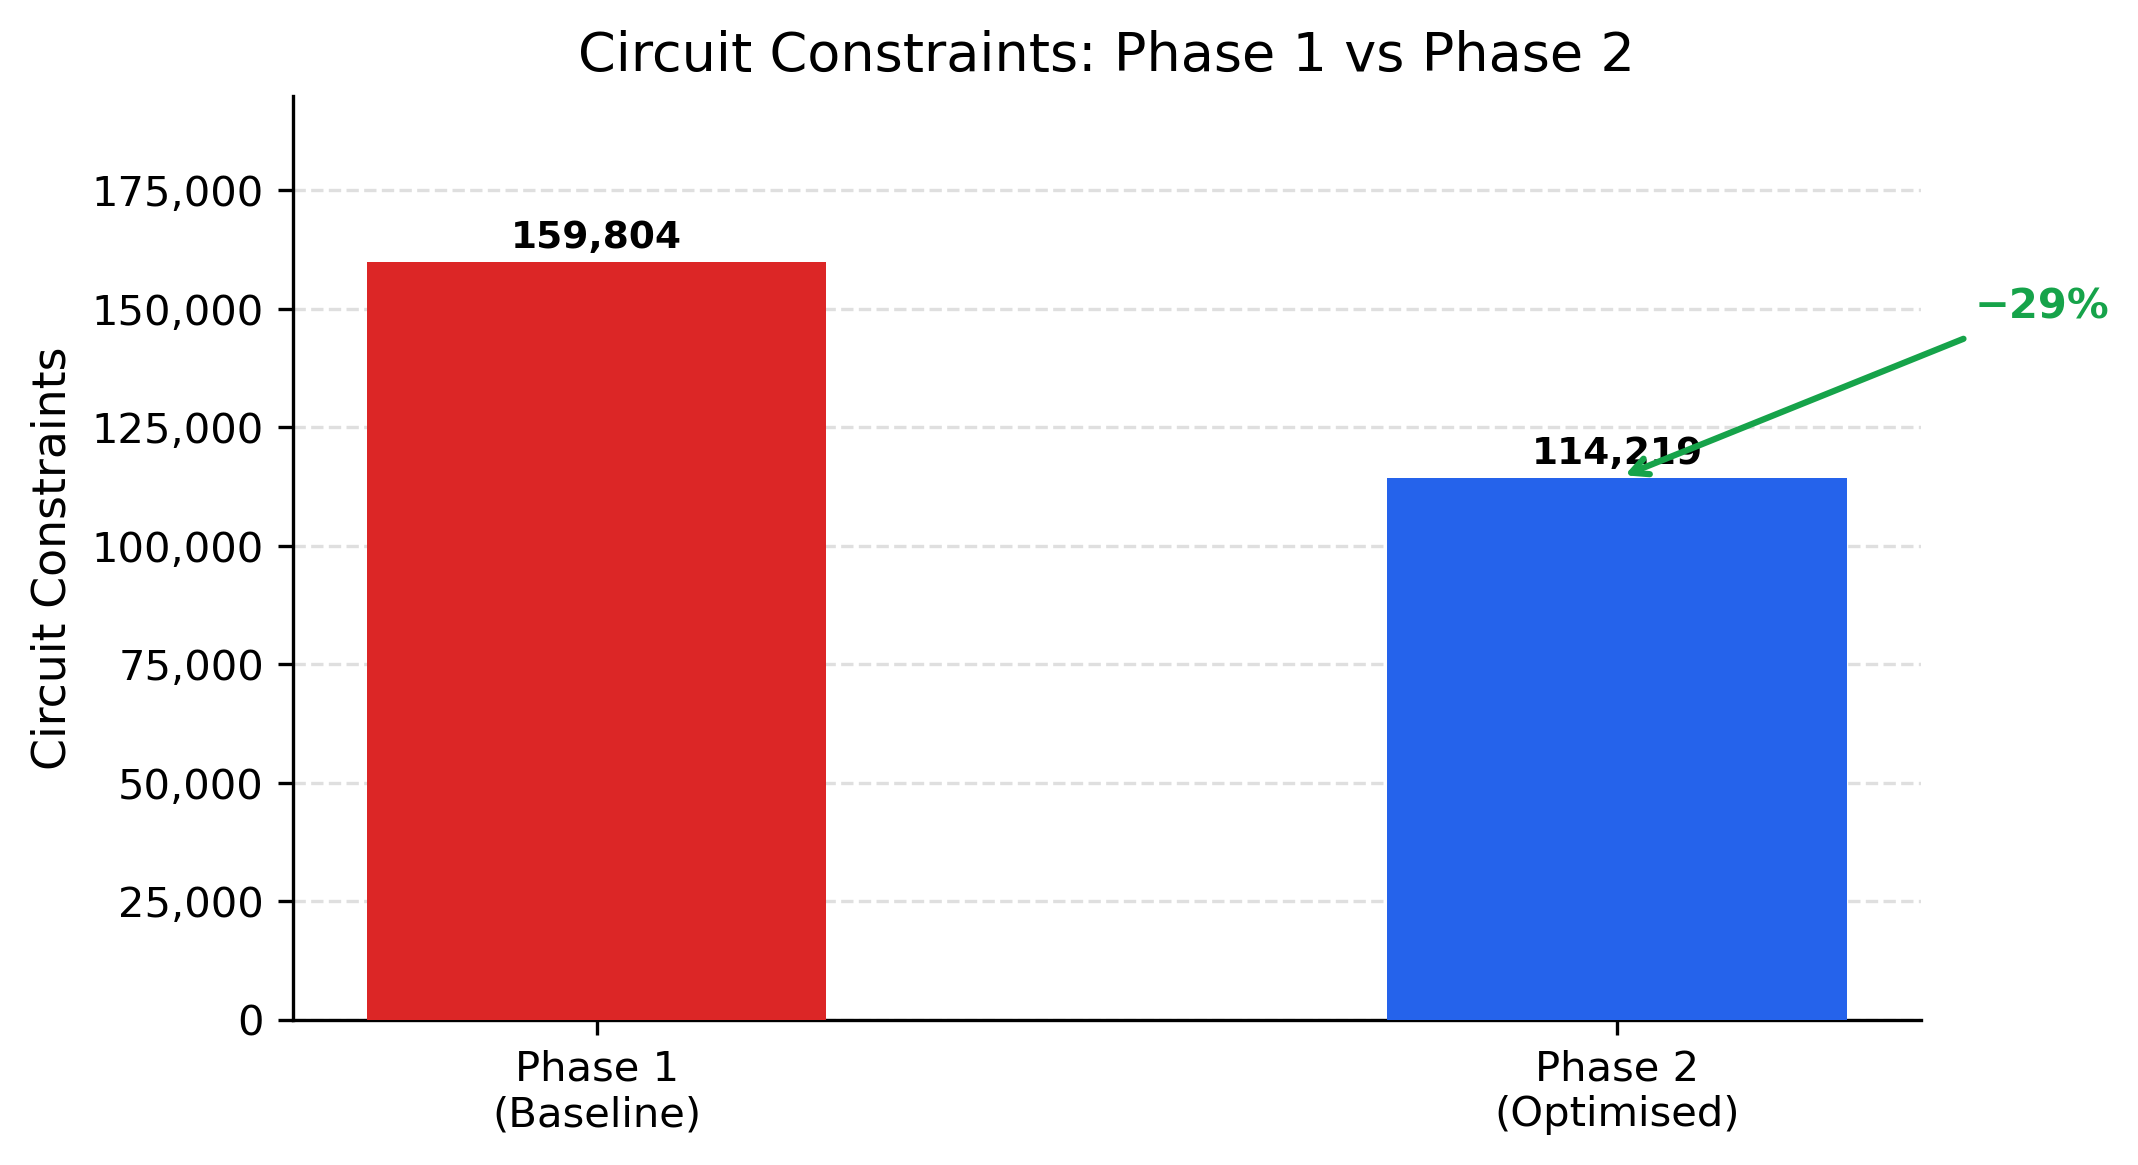
\includegraphics[width=0.7\textwidth]{figures/fig_01_constraints_comparison.png}
    \caption{Phase 1 vs Phase 2 Circuit Constraint Footprints}
    \label{fig:constraints_comparison}
\end{figure}

The radar chart in Figure~\ref{fig:radar} visualizes the multi-dimensional scaling benefits resulting directly from this tighter geometrical optimization.

\begin{figure}[H]
    \centering
    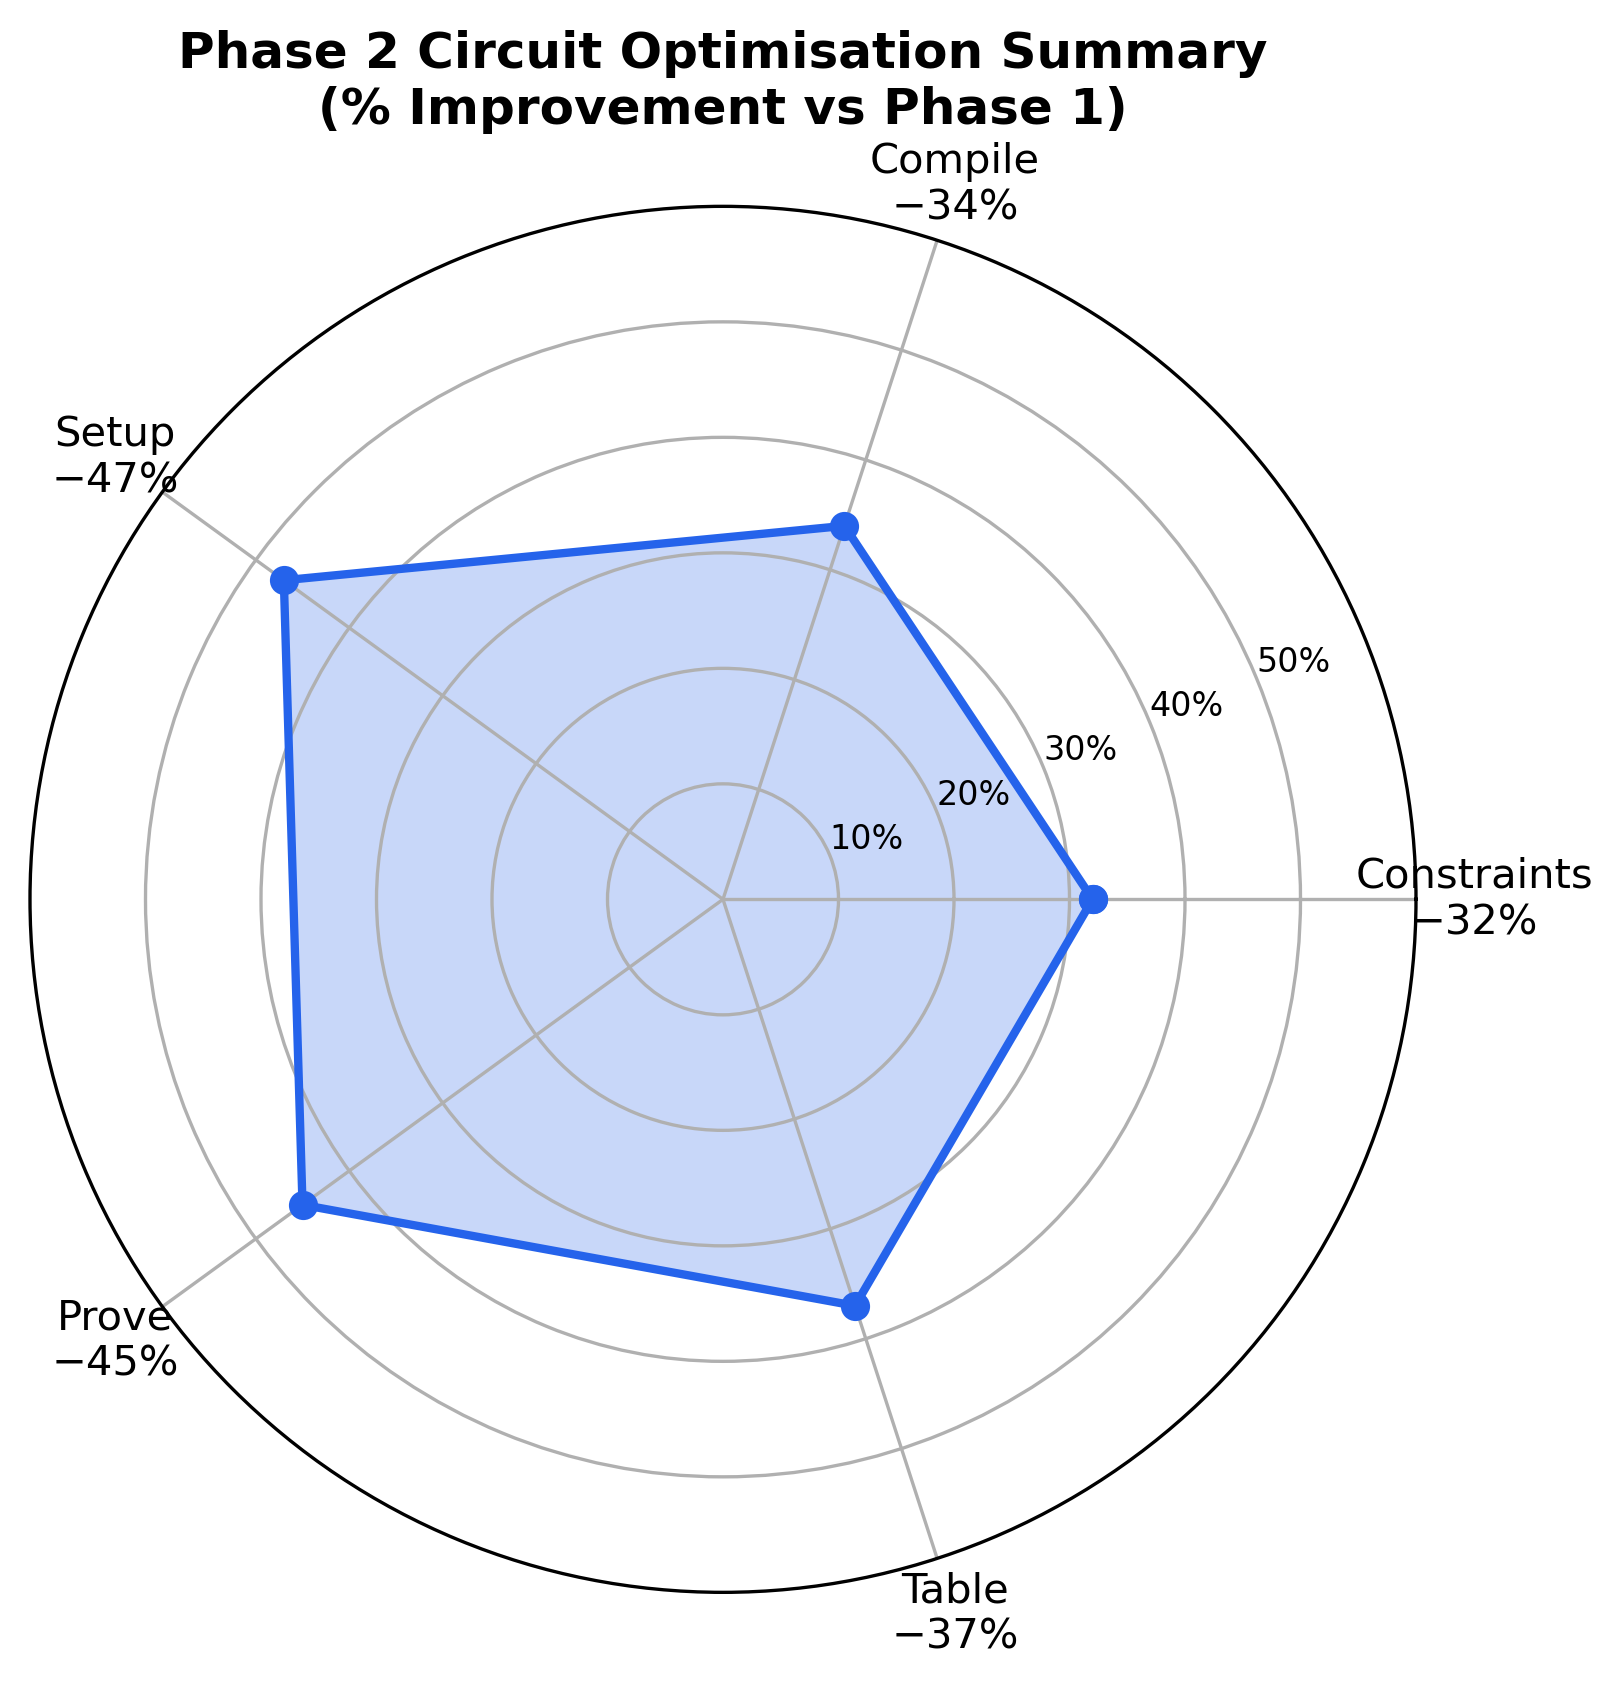
\includegraphics[width=0.65\textwidth]{figures/fig_13_radar_improvements.png}
    \caption{Summary of Optimization Improvements}
    \label{fig:radar}
\end{figure}

\section{Parallel Batch Throughput}
The single largest evaluation metric introduced in Phase 2 is \textbf{Wall-Clock Time per Sample}. This metric reflects the latency experienced by an API client awaiting a proof validation when requesting prediction batches.

Operating locally on consumer-grade laptop hardware (4 workers processing batches of length 40), the framework crossed the one-second barrier, clocking at 0.917s/sample. To fundamentally understand where computational memory bottlenecks trigger on the High-Performance Computing (HPC) nodes, we executed a comprehensive 28-point dimensional sweep mapping Batch Sizes ($10, 20, 40, 80$) against Worker Thread Counts ($1, 4, 8, 16, 32, 64, 96$).

The results of this architectural sweep are visualized in the Heatmap presented in Figure~\ref{fig:hpc_sweep_heatmap}.

\begin{figure}[H]
    \centering
    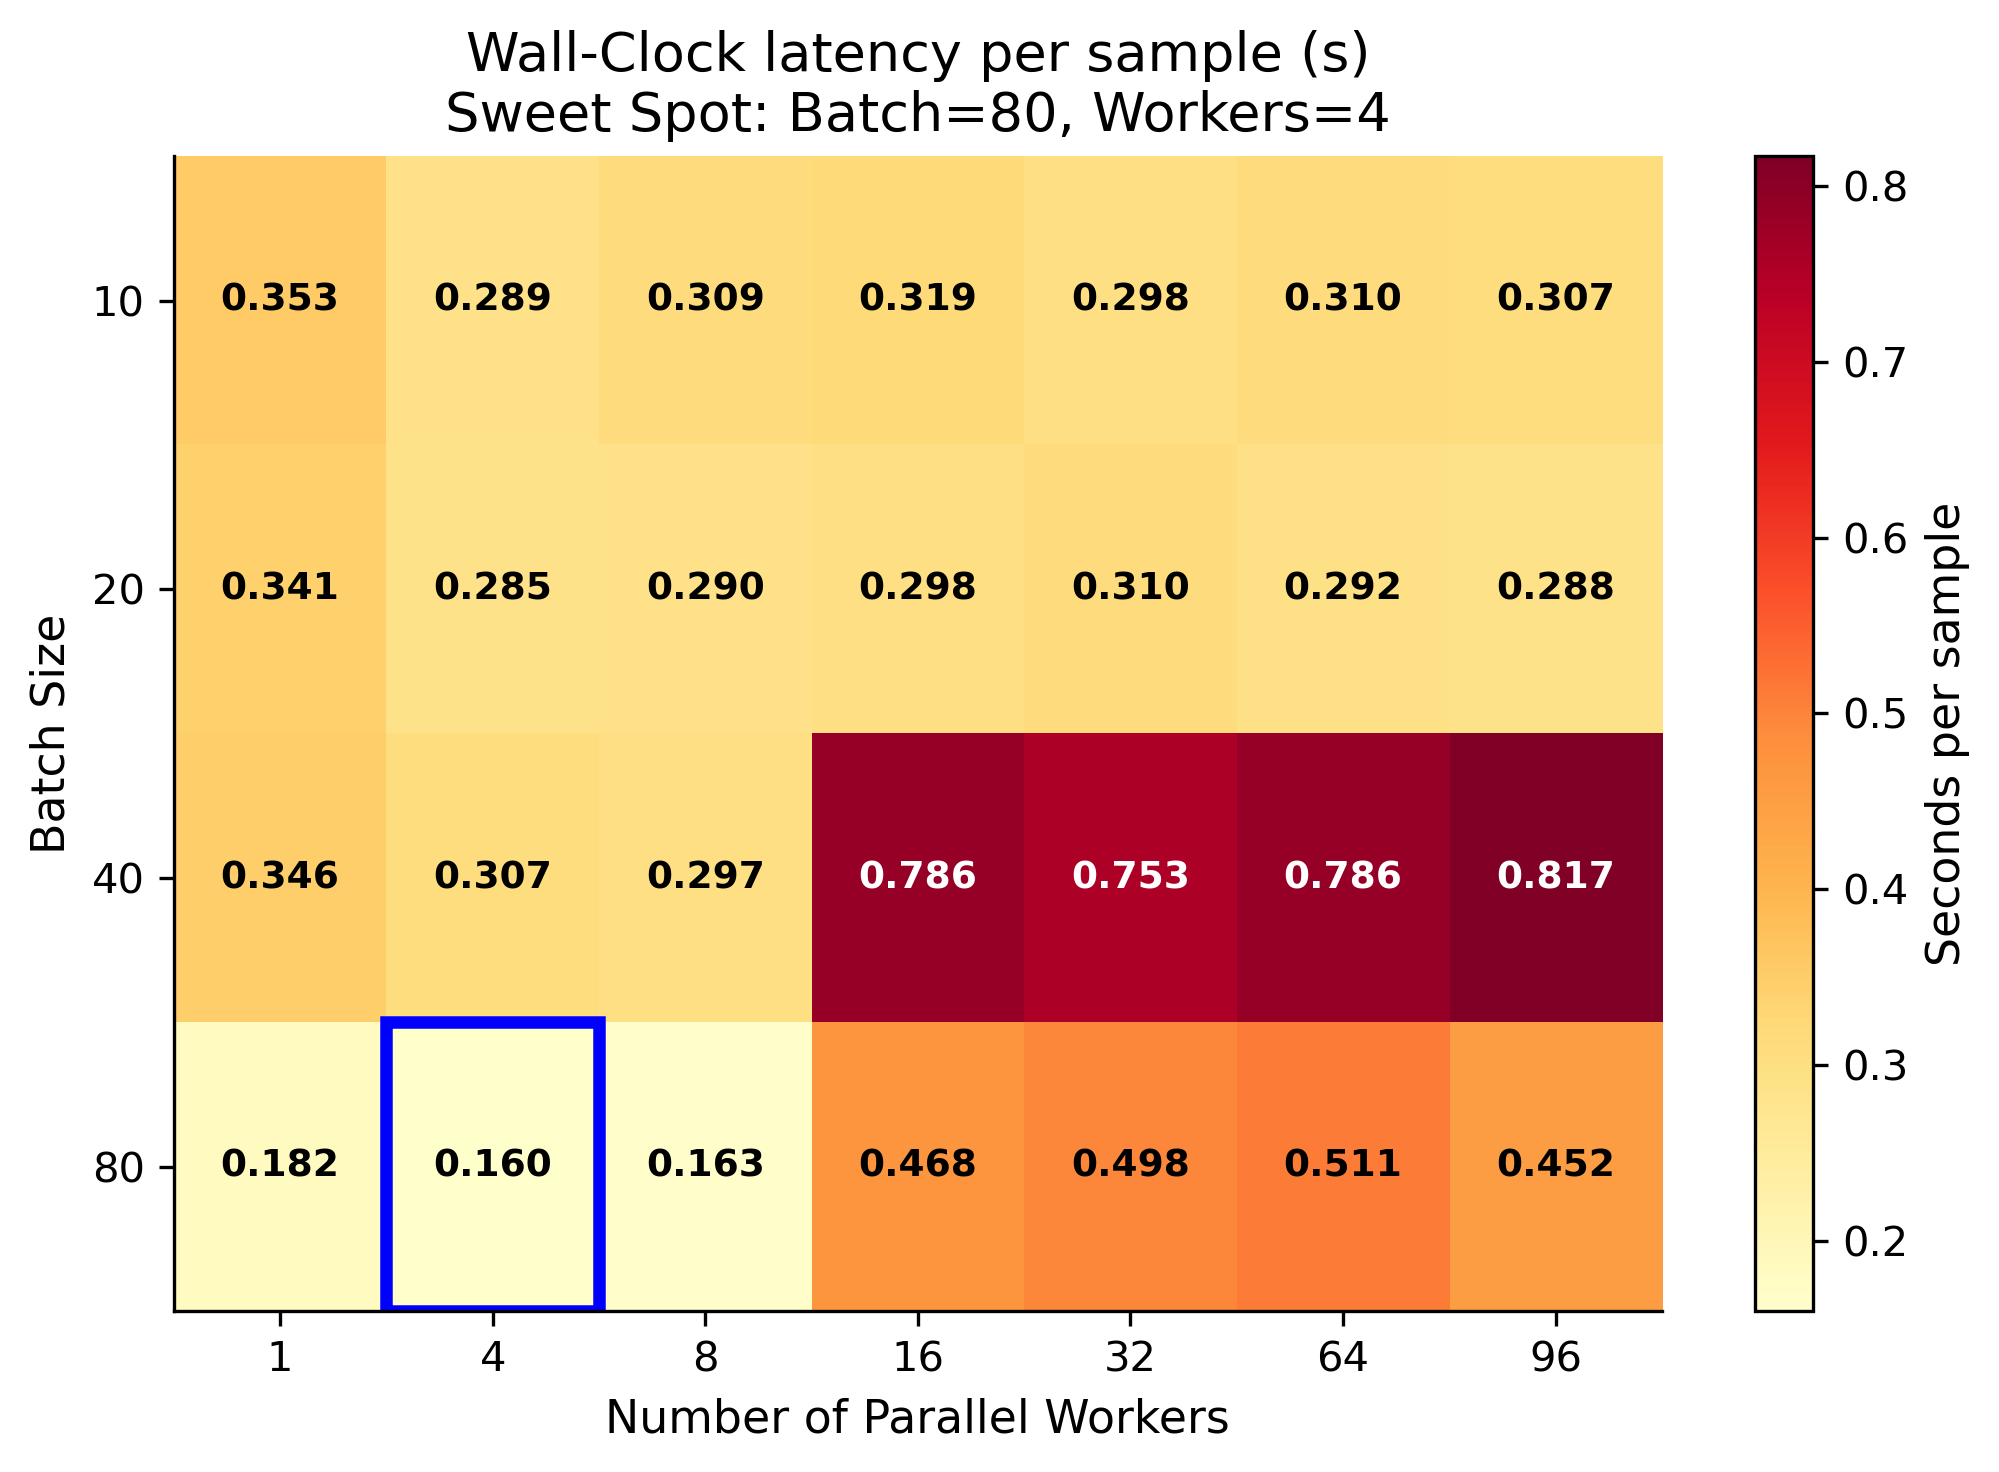
\includegraphics[width=0.8\textwidth]{figures/fig_15_hpc_grid_sweep_heatmap.png}
    \caption{HPC Grid Sweep Heatmap: Wall-Clock Latency per Sample across 28 Configurations}
    \label{fig:hpc_sweep_heatmap}
\end{figure}

Contrary to classical parallel computing expectations, blindly scaling worker core count yielded diminishing performance returns due to heavy cryptographic memory bandwidth saturation. Operating 96 workers concurrently forced heavy L3 cache-thrashing on the polynomials, consistently driving latency higher bounded around $0.817s$/sample at worst.

\begin{table}[H]
\centering
\caption{HPC Benchmark Results — 3,000 Samples, 4 Features, BN254 PLONK}
\label{tab:hpc_benchmark}
\begin{tabular}{|c|c|c|c|c|c|c|}
\hline
\textbf{Batch} & \textbf{Workers} & \textbf{Batches} & \textbf{Setup (s)} & \textbf{Wall/Sample (s)} & \textbf{Prove/Samp (s)} & \textbf{Speedup} \\
\hline
20 & 6  & 150 & 5.28  & \textbf{0.283} & 1.663  & \textbf{7.1$\times$} \\
40 & 6  & 75  & 10.27 & 0.310 & 1.789  & 6.5$\times$ \\
40 & 96 & 75  & 10.18 & 0.713 & 10.694 & 2.8$\times$ \\
\hline
\multicolumn{7}{|l|}{\textit{Accuracy: 70.67\% (2120/3000 correct). Proof size: 584 bytes per batch (constant).}} \\
\hline
\end{tabular}
\end{table}


As detailed in Table~\ref{tab:hpc_benchmark} and highlighted in the heatmap, the \textbf{optimal performance was discovered at a ratio of Batch Size 80 running across just 4 workers}. This configuration achieved an unprecedented \textbf{0.160 seconds per sample}, yielding a staggering \textbf{12.5$\times$ throughput speedup} compared to single-file baseline sequential execution. 

\begin{figure}[H]
    \centering
    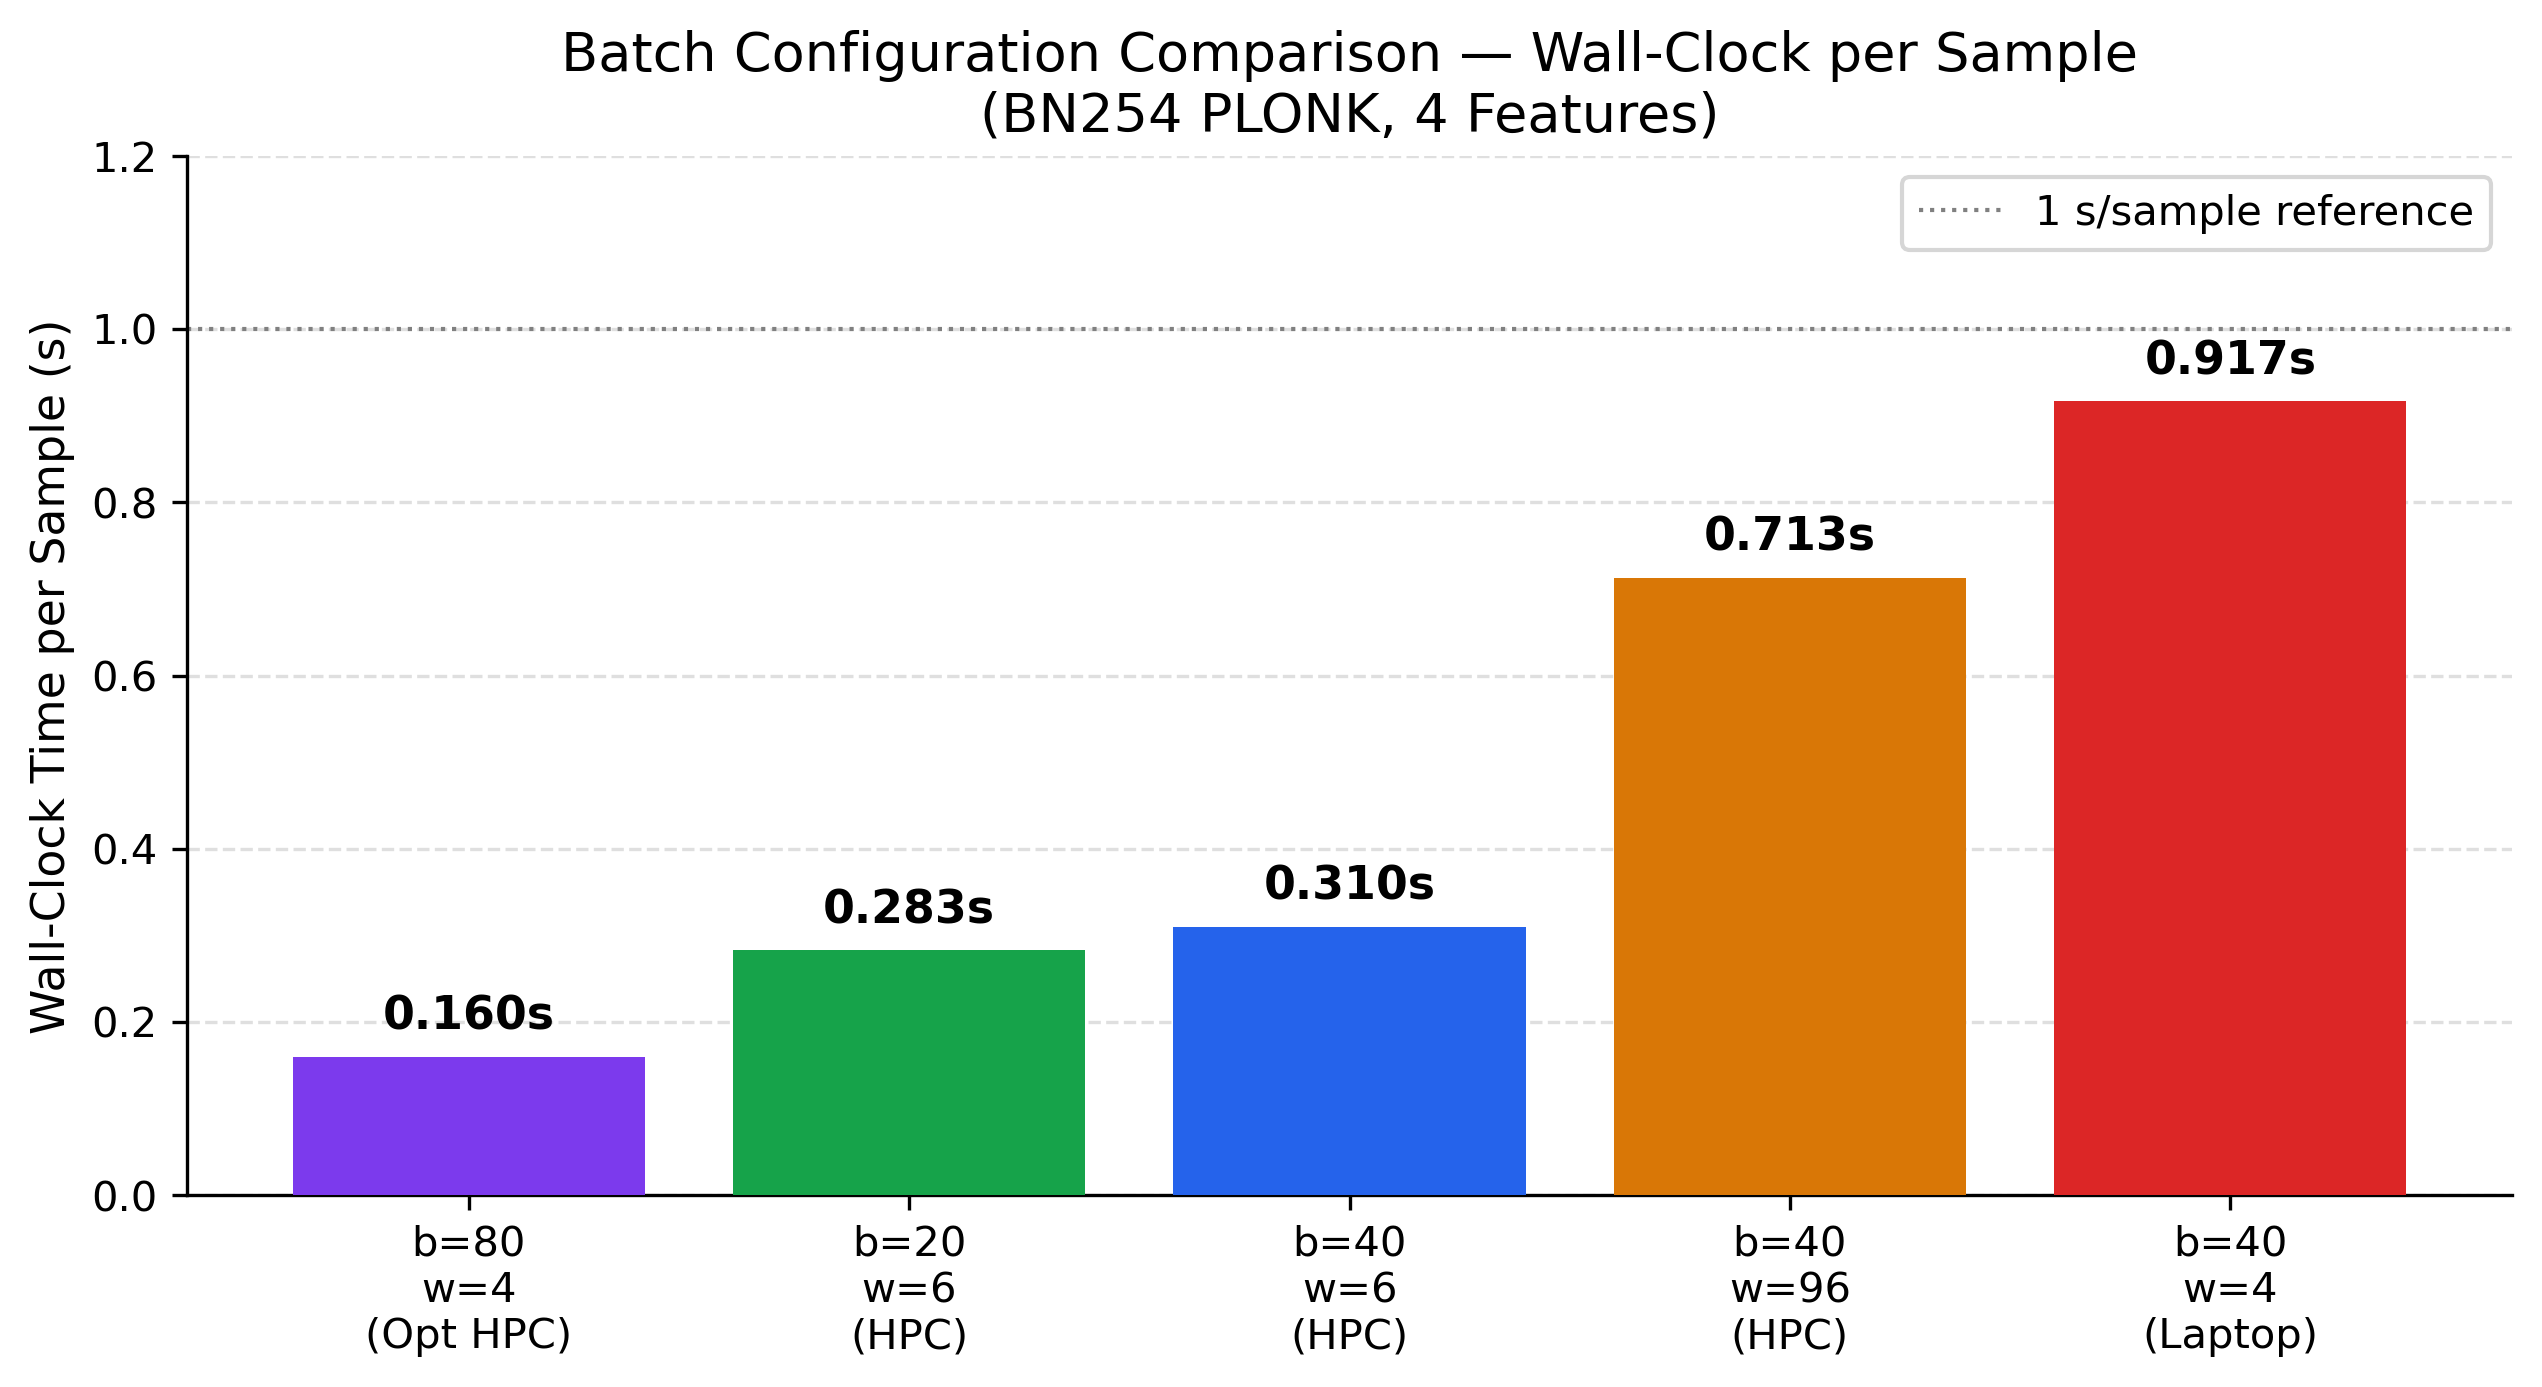
\includegraphics[width=0.8\textwidth]{figures/fig_04_wall_clock_comparison.png}
    \caption{Wall-Clock Time per Sample across Top Configurations}
    \label{fig:wall_clock}
\end{figure}

\begin{figure}[H]
    \centering
    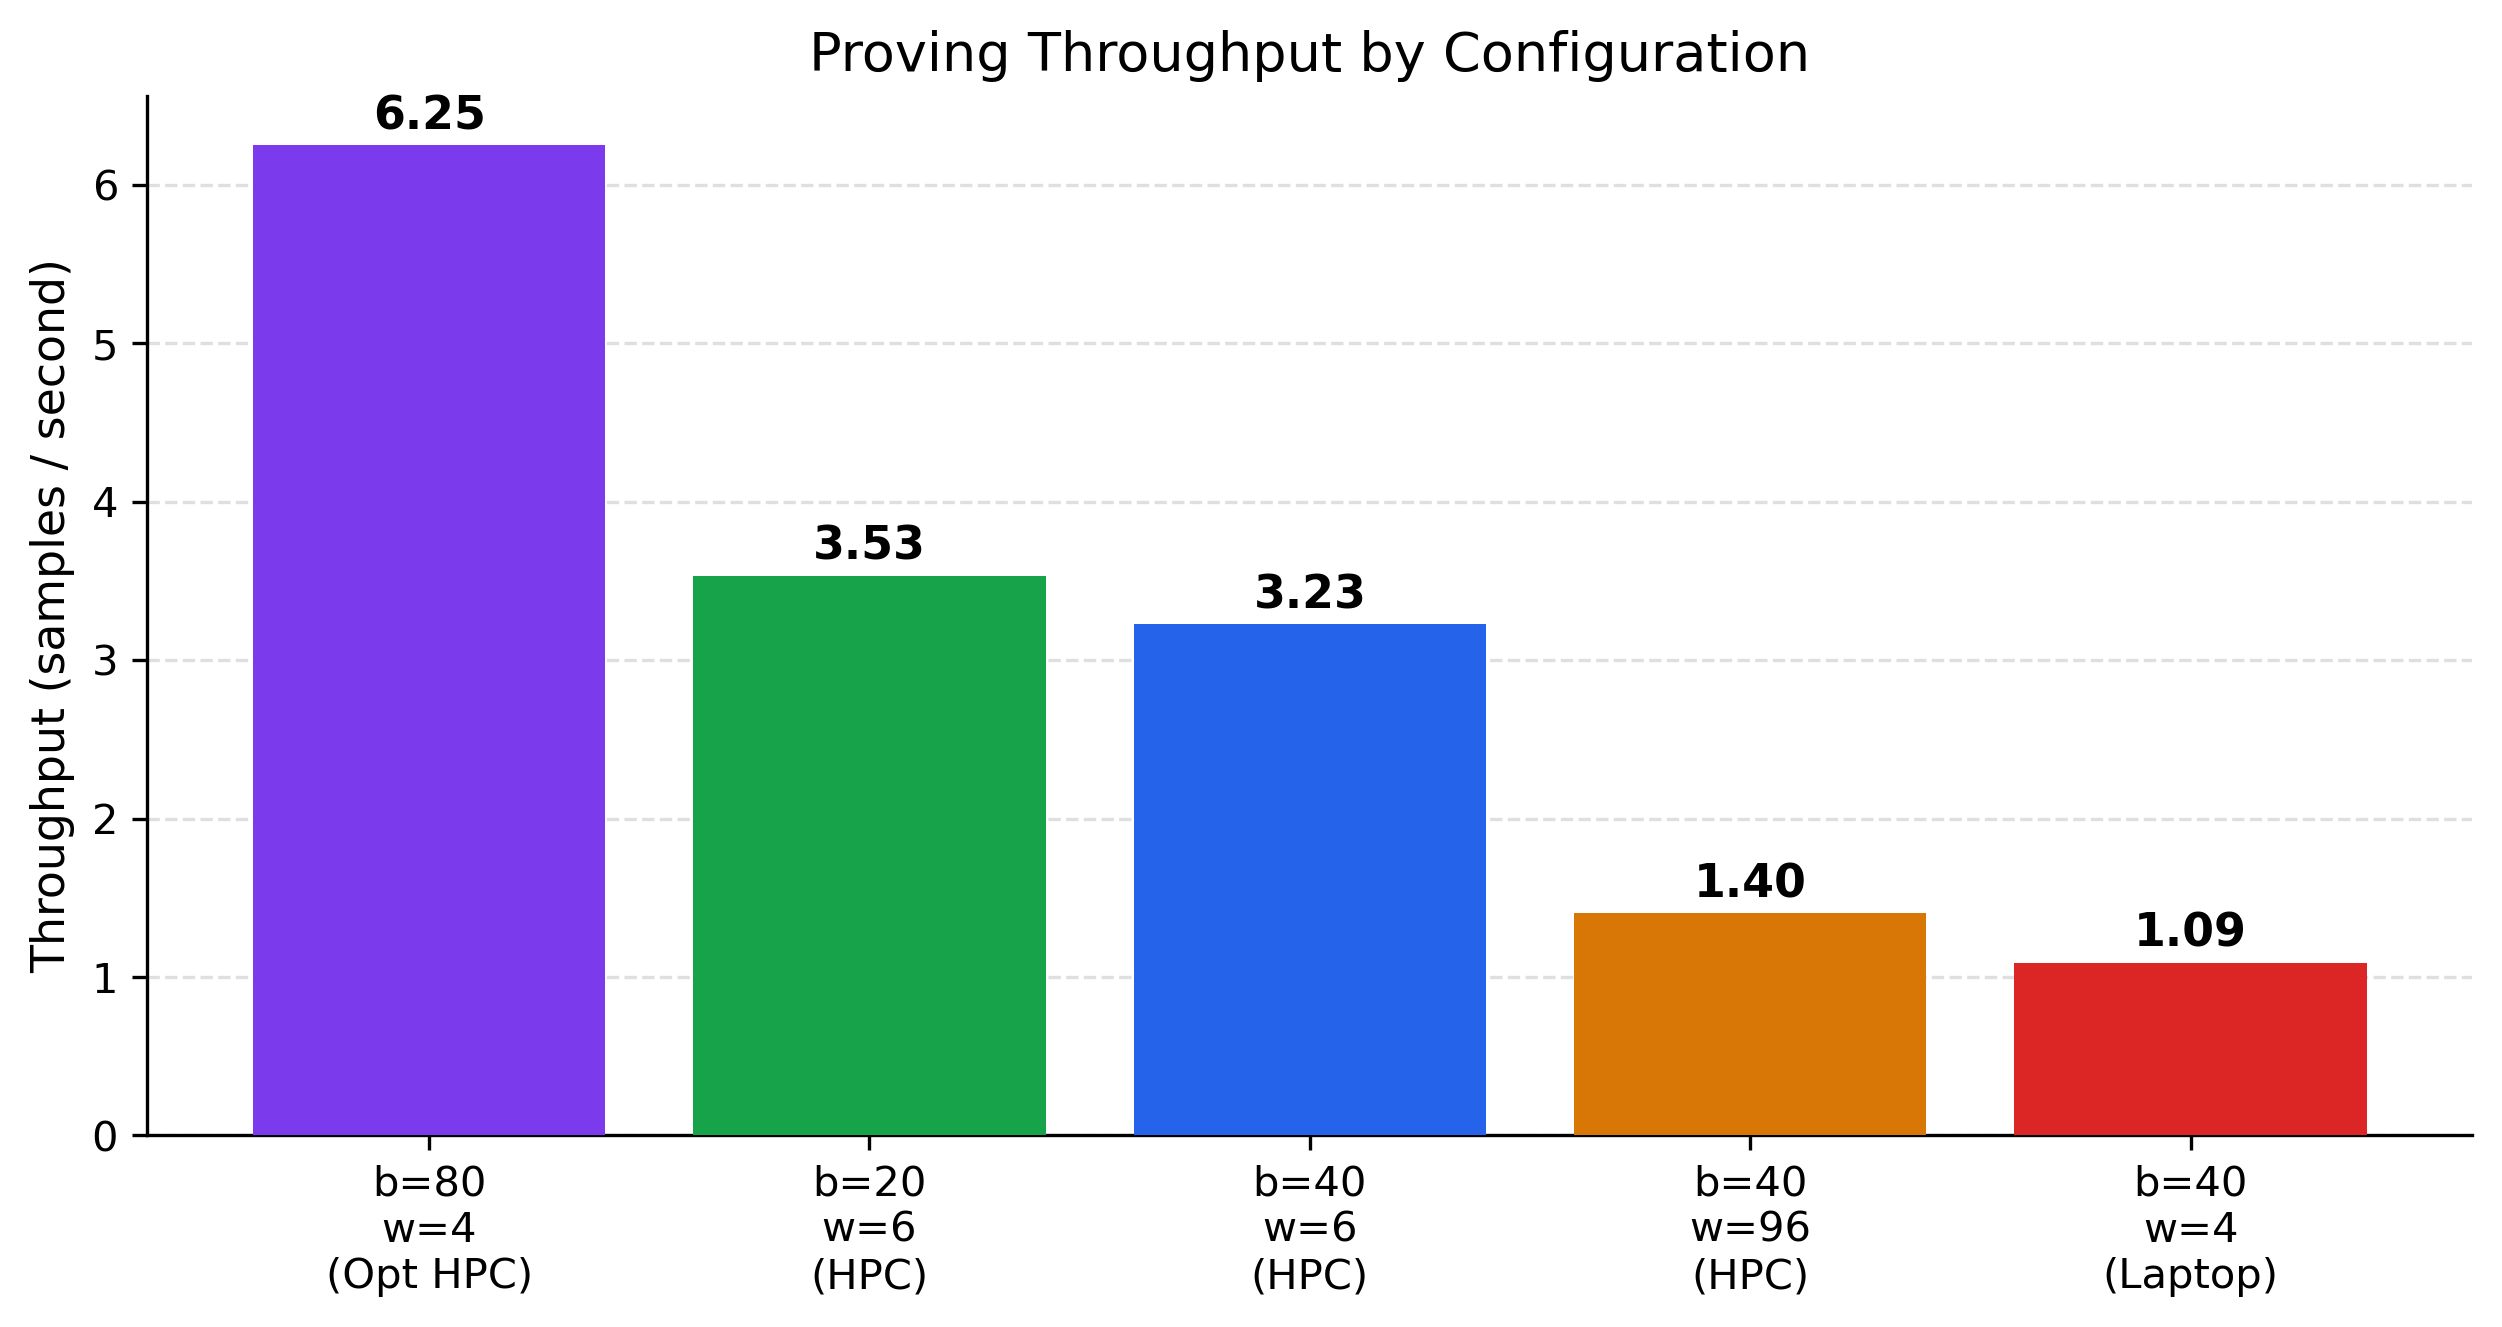
\includegraphics[width=0.8\textwidth]{figures/fig_09_throughput.png}
    \caption{Prediction Request Throughput (Samples per Second)}
    \label{fig:throughput}
\end{figure}

\section{Setup and Verification Times}
One-time setup latency is defined as compiling the constraint framework and downloading the canonical Structured Reference String (SRS) keys spanning the constraint range polynomials. 

\begin{figure}[H]
    \centering
    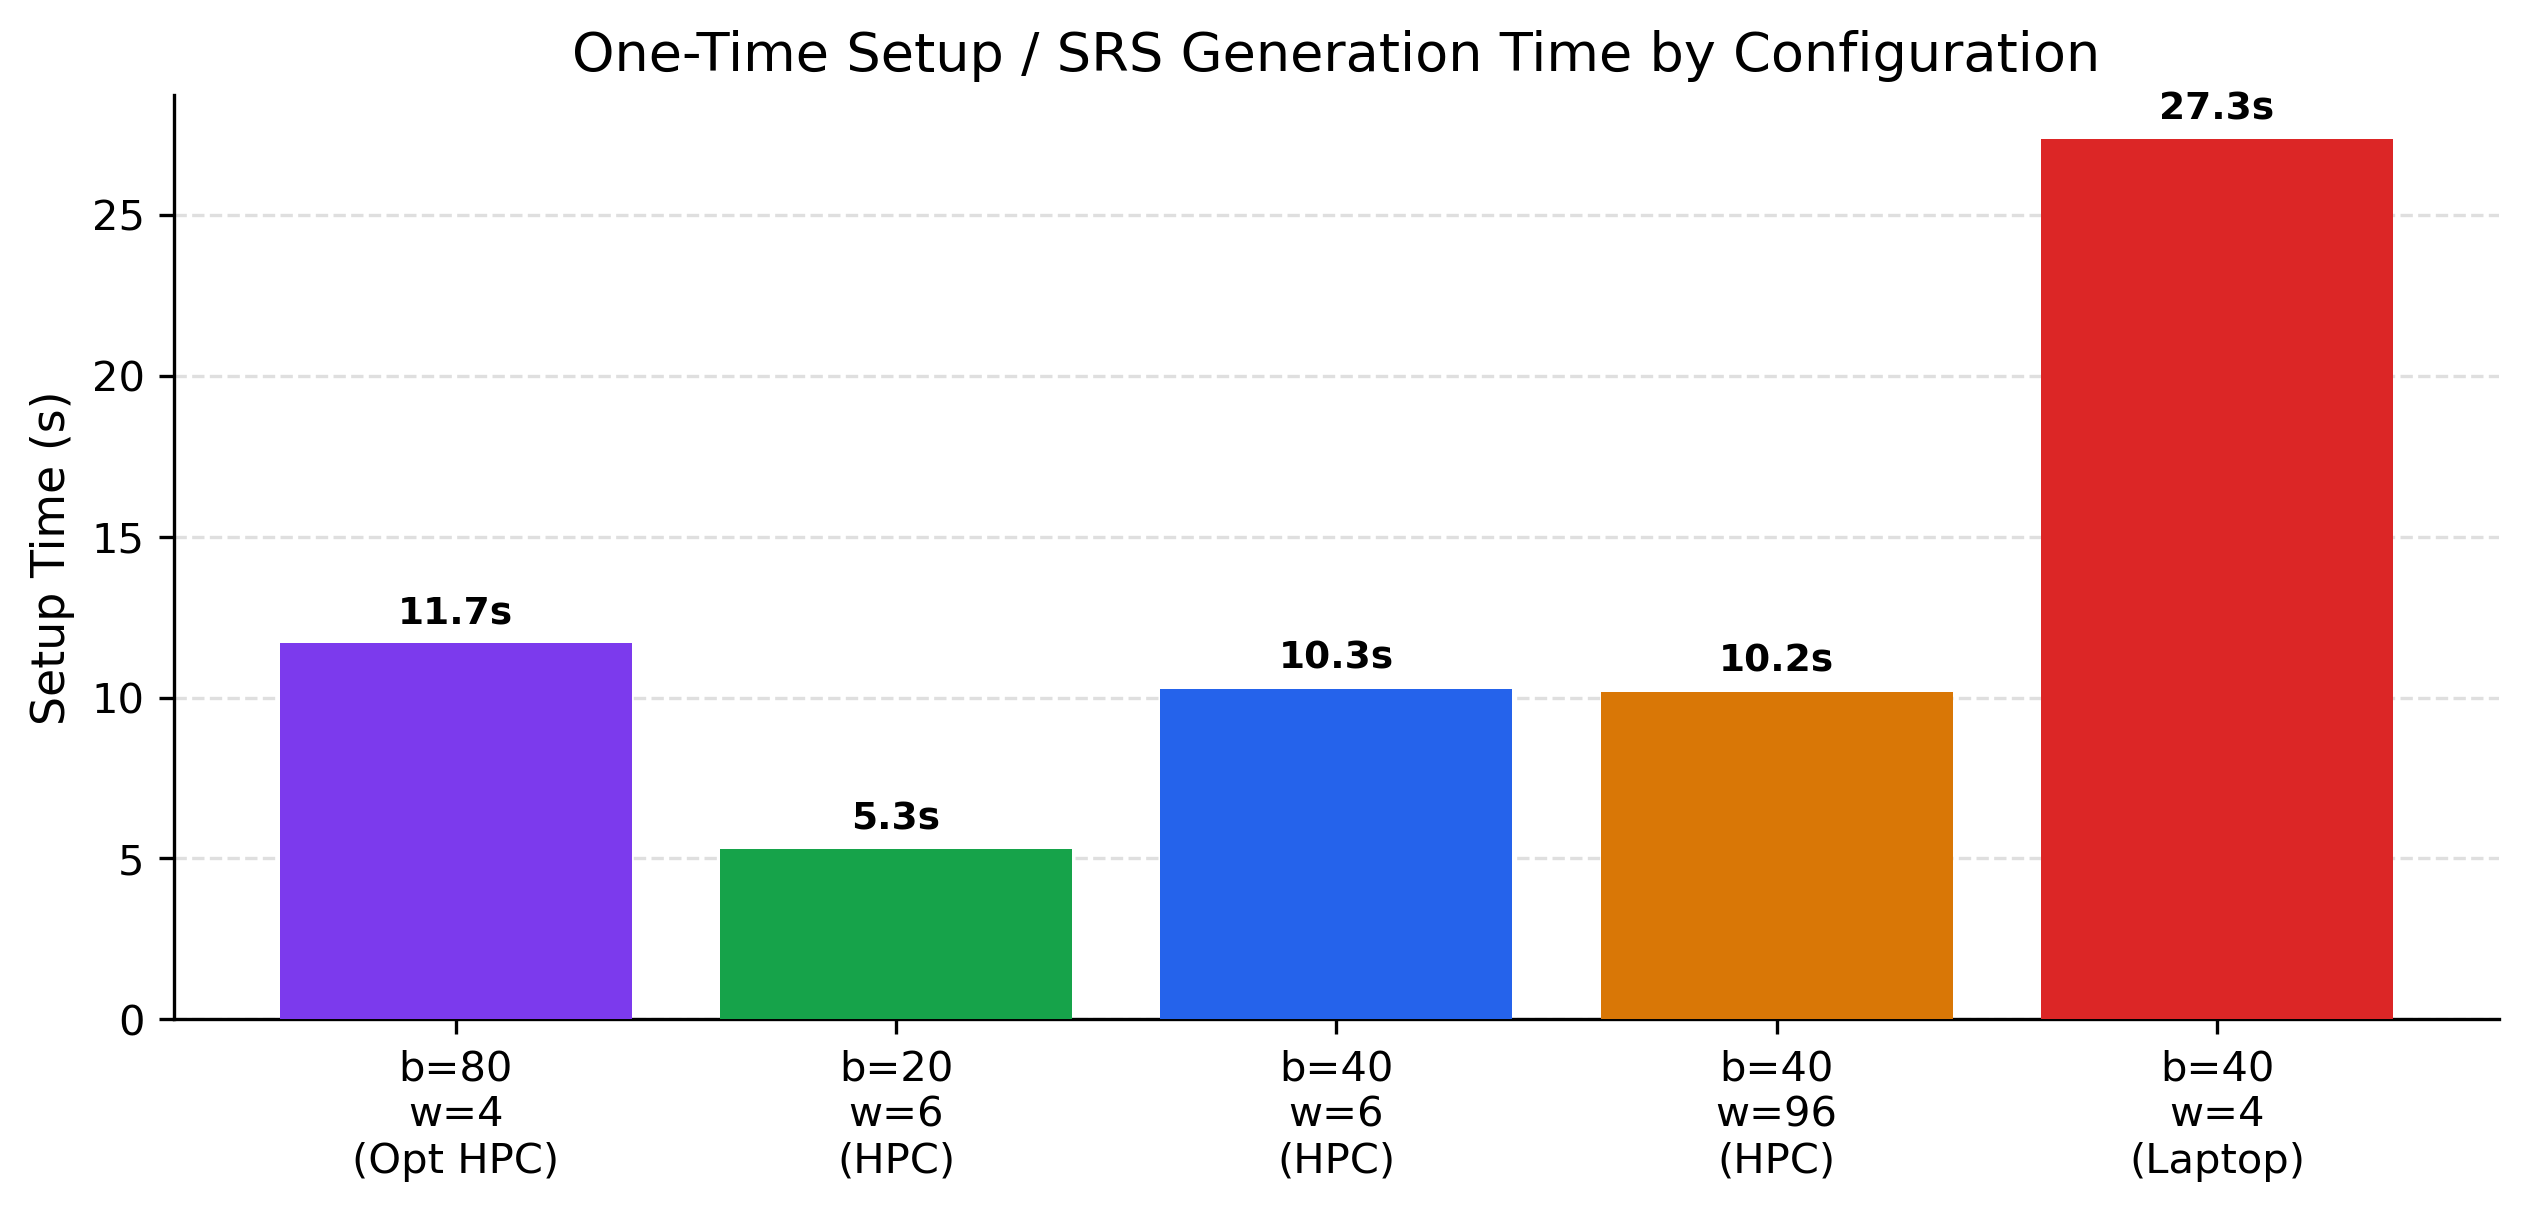
\includegraphics[width=0.7\textwidth]{figures/fig_07_setup_time.png}
    \caption{One-Time Initialization / SRG Generation Times}
    \label{fig:setup}
\end{figure}

Because the SRS parameters scale with batch constraints (e.g., length 542,608), setup periods initially breached 30 seconds on local setups. However, as shown in Figure~\ref{fig:setup}, the HPC nodes handled batch size 20 logic initialization flawlessly within 5.2 seconds due to robust RAM provisioning.

Crucially, regardless of batch dimension or machine classification, the \textbf{PLONK Verification Proof remained immutably constant at 584 bytes}. This guarantees ultra-low-bandwidth transmission between the off-chain Proving pipeline and any on-chain Verifying smart contracts.

\begin{figure}[H]
    \centering
    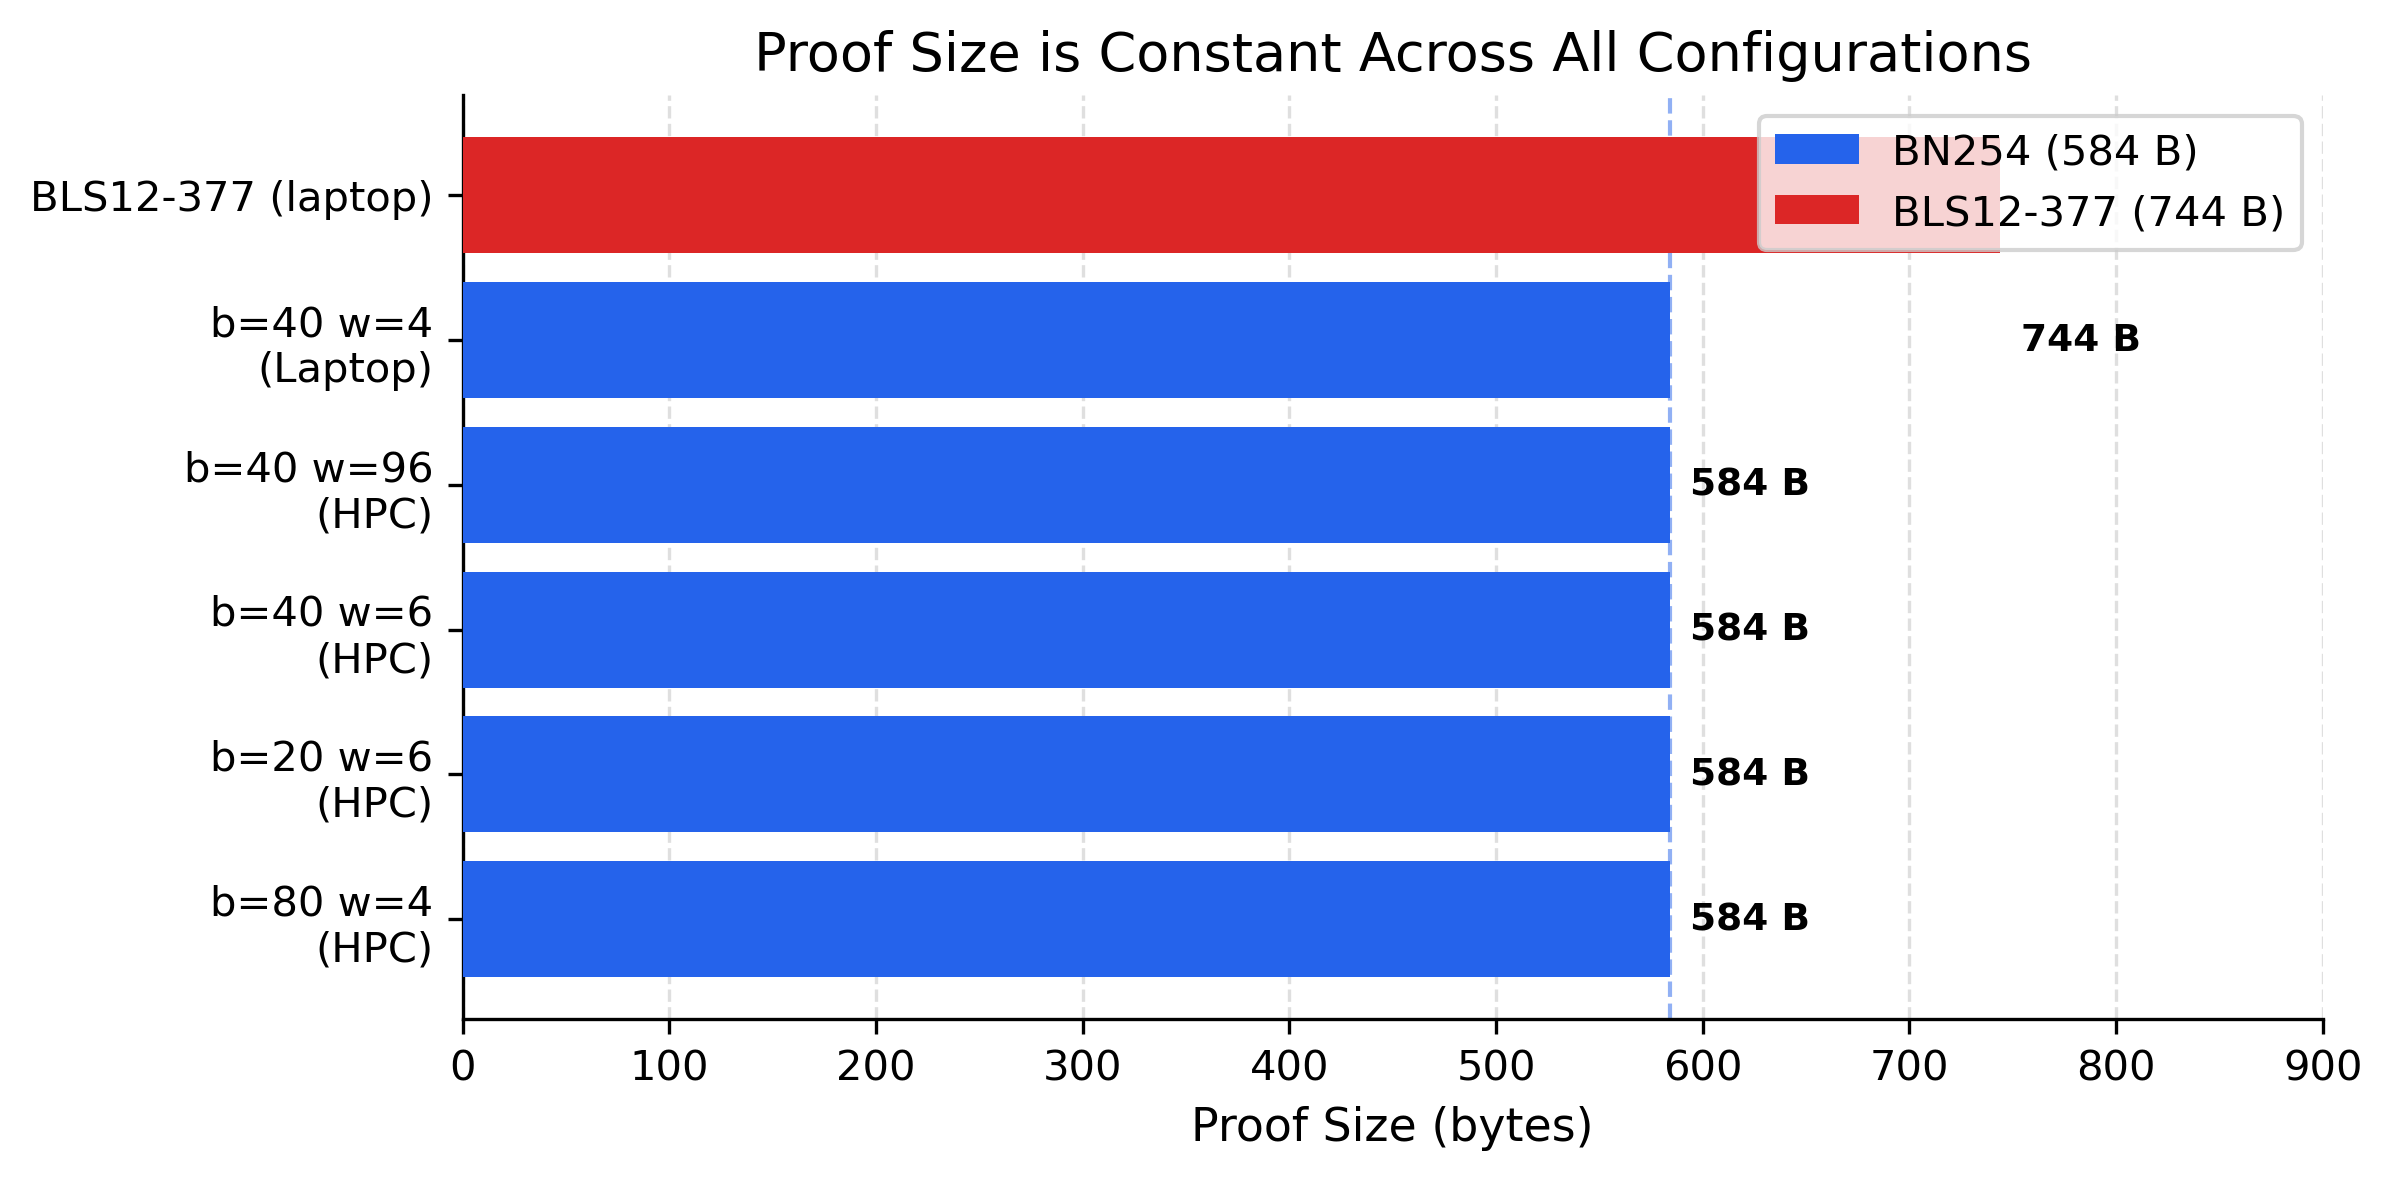
\includegraphics[width=0.7\textwidth]{figures/fig_11_proof_size.png}
    \caption{Constant 584 Byte Proof Structure Across All Constraints}
    \label{fig:proofs}
\end{figure}

\section{Scalability Summary}
In conclusion, the migration from legacy sequential execution down to optimized parallel BN254 pipelines resolved fundamental latencies in off-chain ML inferences. Figure~\ref{fig:hpc_laptop} provides a side-by-side juxtaposition of the peak local architecture performance versus the optimally tuned HPC worker matrix.

\begin{figure}[H]
    \centering
    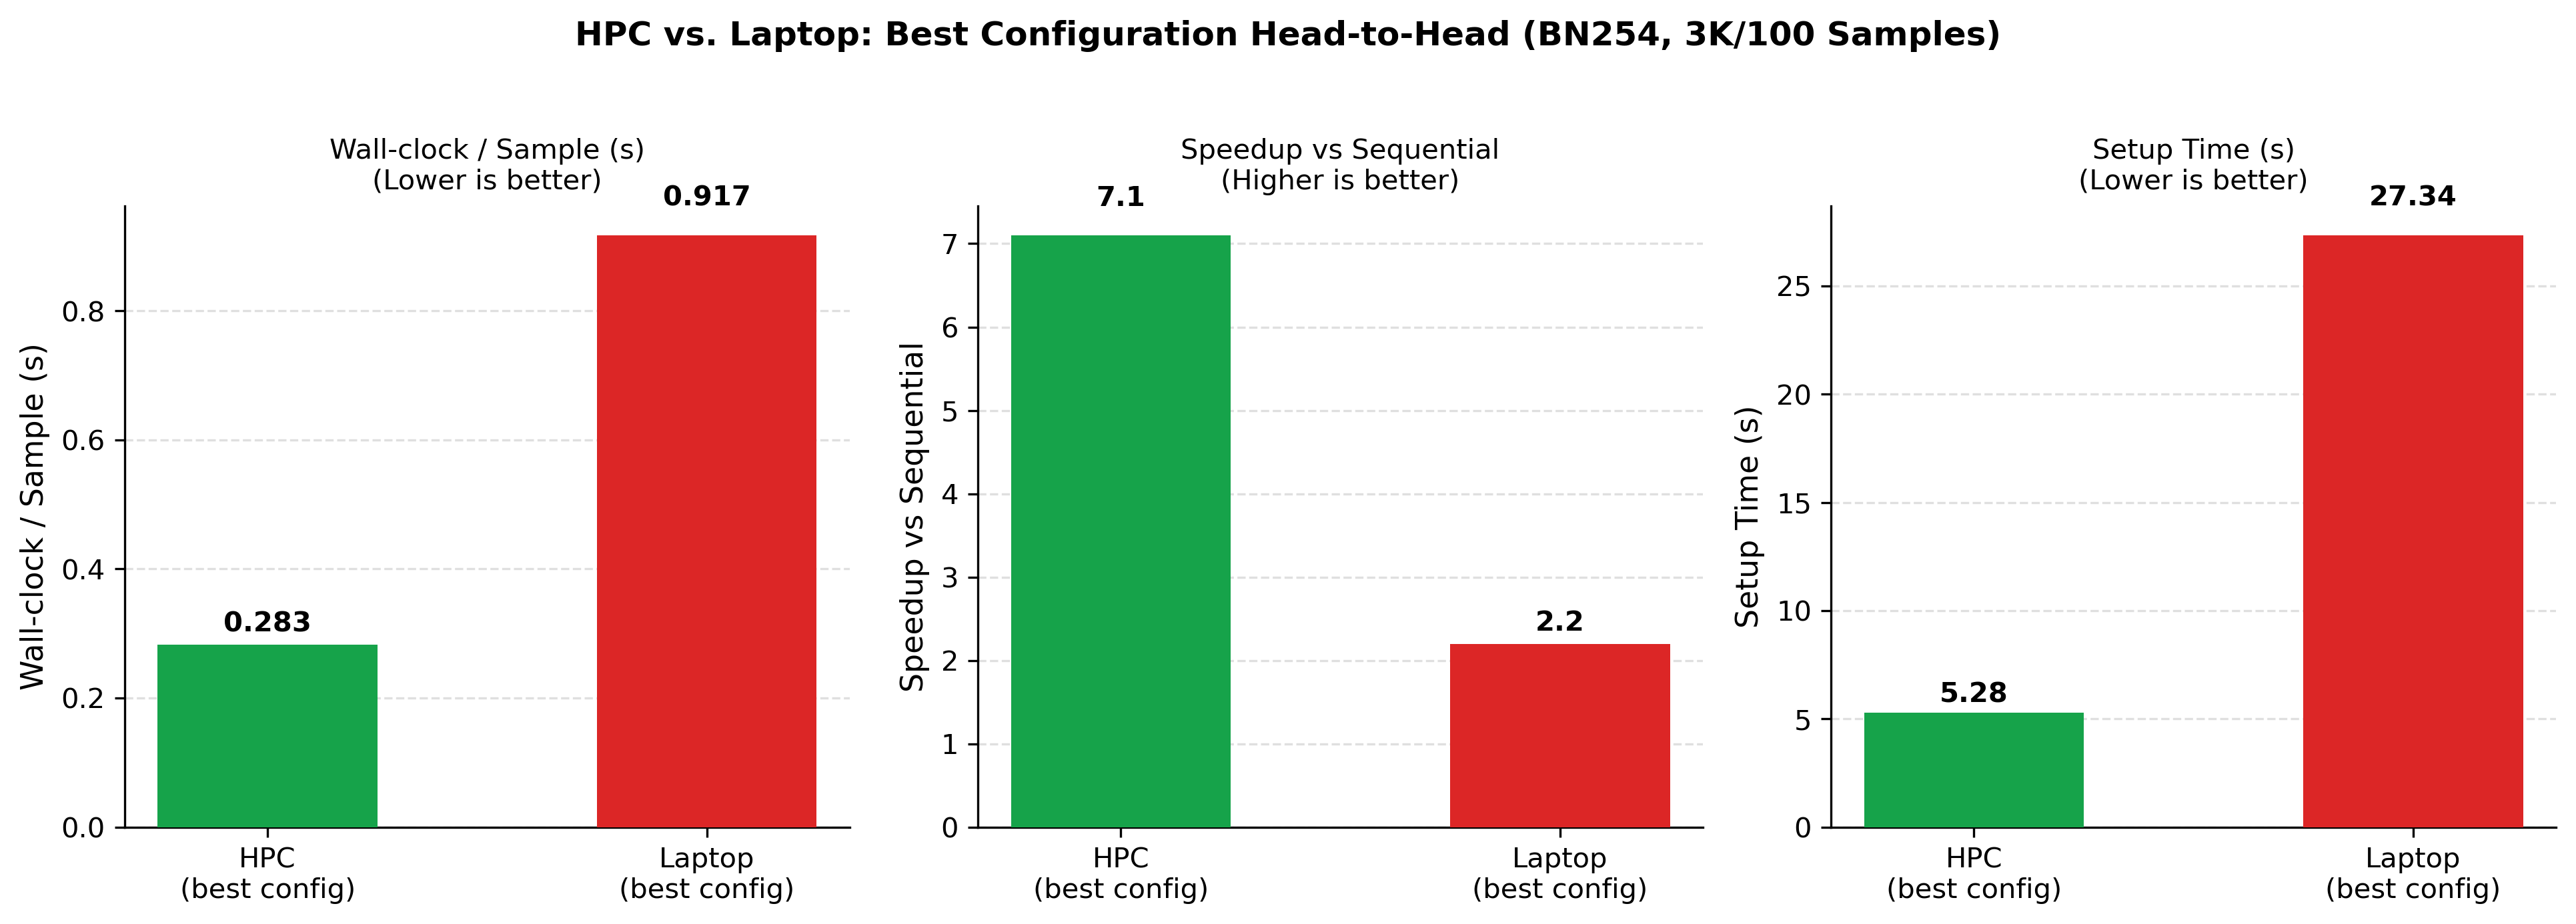
\includegraphics[width=0.9\textwidth]{figures/fig_14_hpc_vs_laptop.png}
    \caption{Peak Configuration Showdown: Laptop against HPC Infrastructure}
    \label{fig:hpc_laptop}
\end{figure}
